\documentclass[../../main.tex]{subfiles}

\graphicspath{{../../fig/}}
\setcounter{section}{0}

\begin{document}
\chapter{スパースワイヤーグリッドのたわみ量の評価}
\label{chap:wiresag_swg}
\ref{}章にて、ワイヤーのたわみ量を自動で評価する装置を開発した。
本章では、開発した装置を用いて実際に偏光角較正に使用されるスパースワイヤーグリッドのたわみ量を評価する。
はじめに、評価するスパースワイヤーグリッドの作成方法について述べ、次いで評価結果とその考察を行う。
その後、評価されたたわみ量が大きかったものについて修繕を加え、再度評価を行った結果について述べる。
最後に、今回のたわみ量の評価を通じて得られた、スパースワイヤーグリッドの作成方法に関する今後の展望について述べる。

\section{評価されたスパースワイヤーグリッドの詳細}
今回評価したスパースワイヤーグリッドは、\ref{subsec:wg_design}項で述べたように$\SI{230}{g}$の重りを使用し、
ワイヤー番号が奇数番目のものと偶数番目のものに分け、二回に分けてワイヤーを張ることで作成された。
作成されたスパースワイヤーグリッドを装置に取り付けた様子を図\ref{fig:wiresag_sparse_wiregrid}に示す。
なお、\ref{chap:wiresag}章にて述べたように一度に測定できるのはスパースワイヤーグリッドの半面のみであるので、
ワイヤー番号が$0\sim19$のワイヤーと$20\sim38$のワイヤーに分けて測定を行った。
\begin{figure}[tbp]
    \centering
    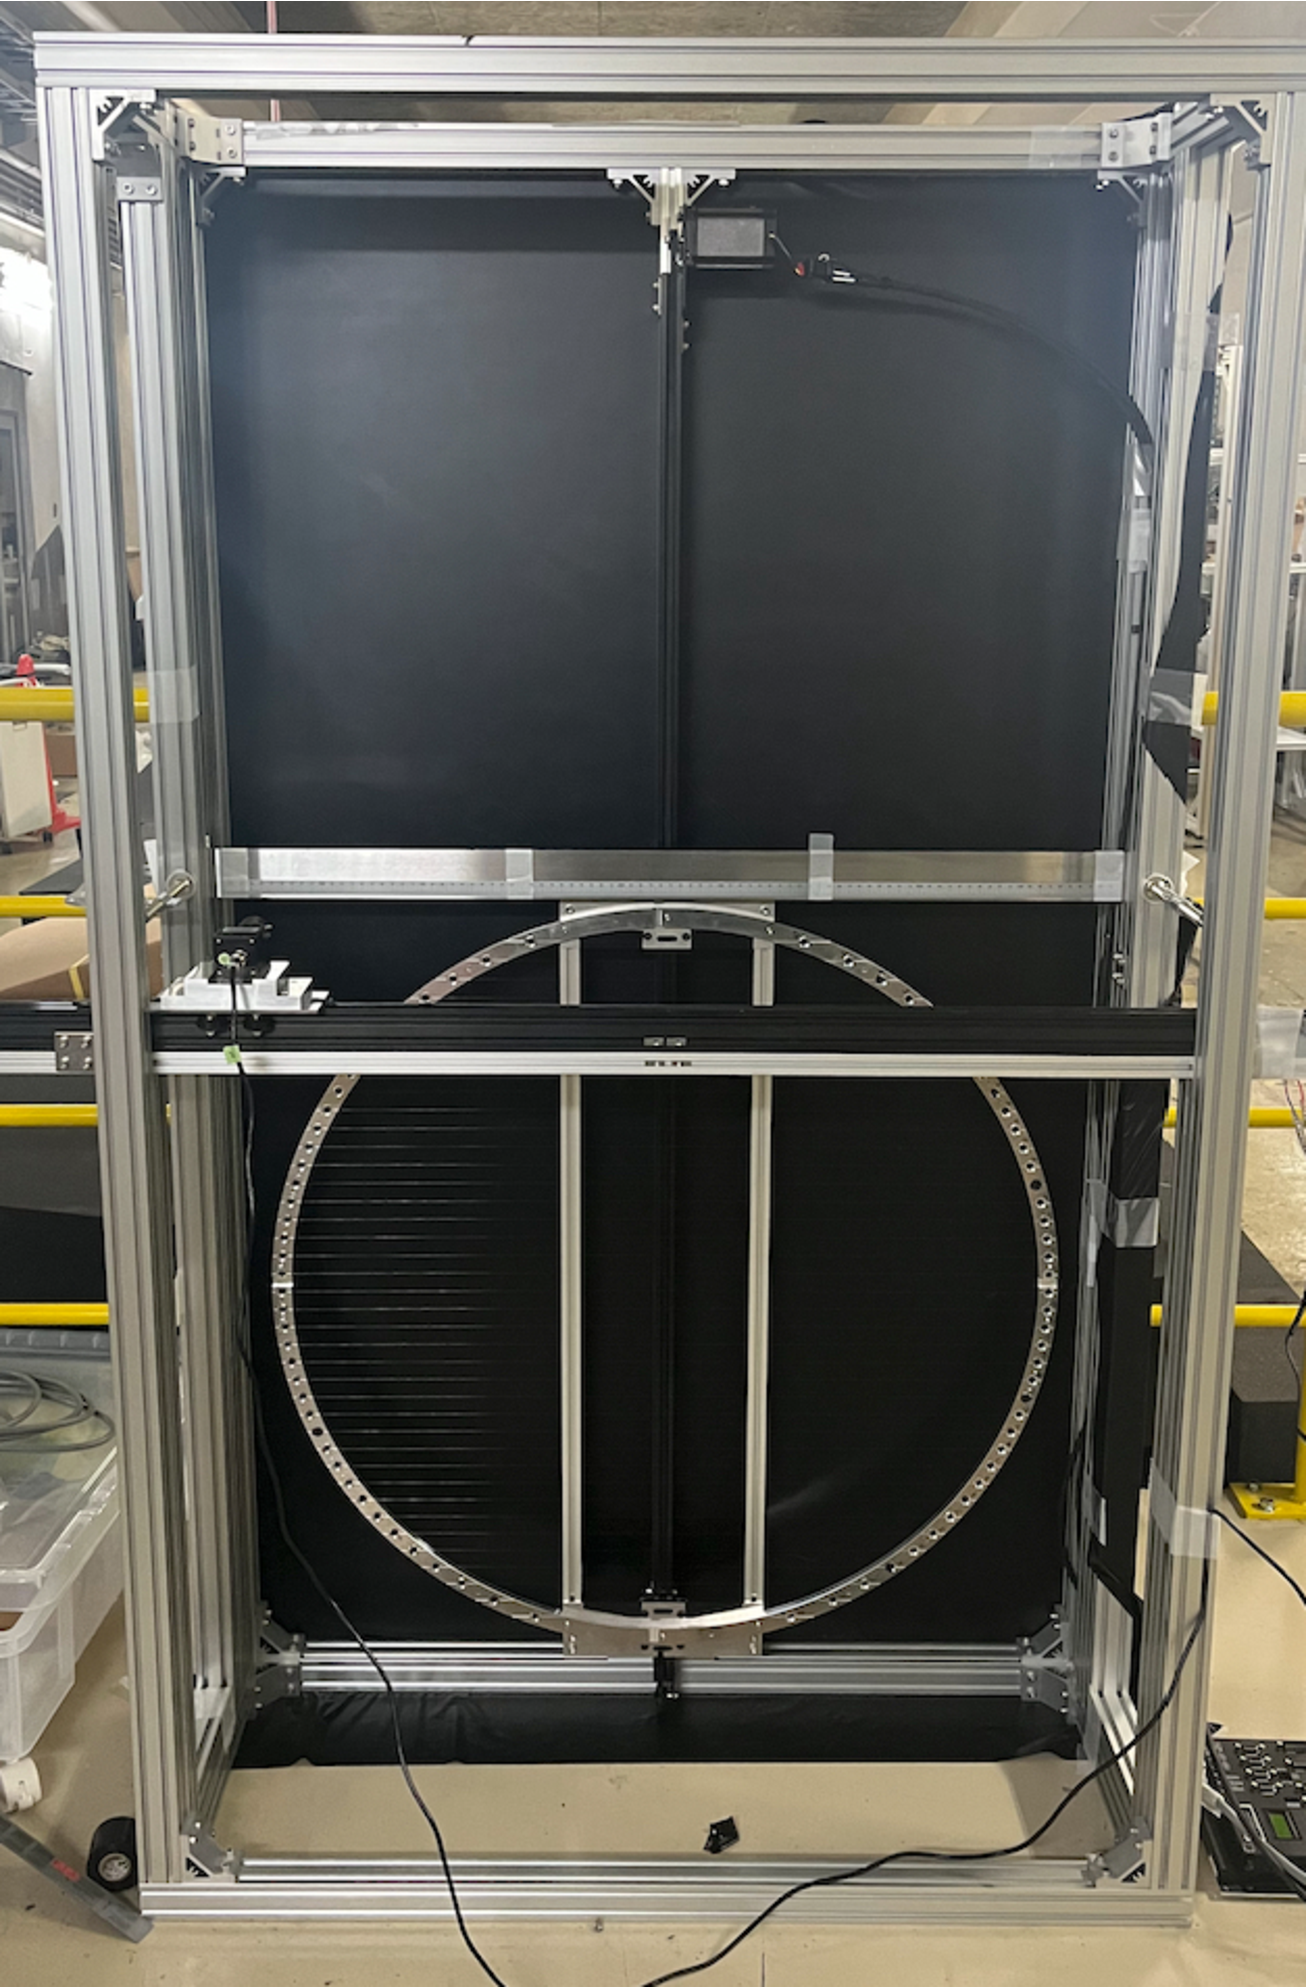
\includegraphics[width=0.6\textwidth]{wiresag_swg/wiresag_sparse_wiregrid.pdf}
    \caption{スパースワイヤーグリッドのたわみ量の評価の様子}
    \label{fig:wiresag_swg_sparse_wiregrid}
\end{figure}
\subsection{評価結果とその考察}
図\ref{fig:wiresag_swg_sparse_wiregrid_result}にスパースワイヤーグリッドのたわみ量の評価結果を示す。
横軸はワイヤー番号、縦軸はワイヤーのたわみ量を示している。
また、図\ref{}には評価されたたわみ量をたわみ角に変換した結果を示す。


\end{document}